
In this work, we are quantifying the effect of super-sample effect on the covariance matrix of higher-order statistics for a weak lensing survey. To achieve this, we are conducting a series of N-body simulations and analyzing the resulting convergence maps. These maps allow us to compute the statistics and covariance matrices for various statistical measures. Therefore, we can investigate the impact of super-sample covariance on the covariance matrices of these statistics.

In the following sections, we will discuss the methodology used to generate the convergence maps, extract patches for analysis, incorporate noise, apply Gaussian smoothing, and compute the statistical measures. We will also outline the process for estimating the covariance matrices and comparing the results between the BIGBOX and TILED simulations. 

\section{N-body Simulations}
We employed the publicly available particle-mesh simulation code, \texttt{FASTPM} \citep{10.1093/mnras/stw2123} to generate the simulations used in this study. As discussed in Section~\ref{sec:fastpm}, \texttt{FASTPM} is chose to achieve high accuracy while minimizing computational time. 

The two simulations we have used are \textbf{BIGBOX} and \textbf{TILED}. For both simulations, we have used the same cosmological parameters as the IllustrisTNG project \citep{2019ComAC...6....2N}. The parameters are listed in Table~\ref{tab:simulations}. 

\begin{table}[h]
    \centering
    \begin{tabular}{lcc}
    \toprule
    \textbf{Parameter} & \textbf{Symbol} & \textbf{Value} \\
    \midrule
    Hubble constant & $H_0$ & 67.74 \, [$\mathrm{km\,s^{-1}\,Mpc^{-1}}$] \\ 
    Matter density & $\Omega_m$ & 0.3089 \\
    Baryon density & $\Omega_b$ & 0.0486 \\
    Amplitude of fluctuations & $\sigma_8$ & 0.8159 \\
    Spectral index & $n_s$ & 0.9667 \\
    Sum of neutrino masses & $M_{\nu}$ & 0.0 \, [eV] \\
    \bottomrule
    \end{tabular}
    \caption{Cosmological parameters used in the N-body simulations.}\label{tab:simulations}
    \end{table}

The \textbf{BIGBOX} simulation, conducted as part of the HalfDome project \citep{2024arXiv240717462B}, models using $6144^3$ particles, a box with a side length of $3750$ Mpc/h and periodic boundary conditions. We replicated the box $2$ times along each axis ($2^3$ replications in total), in order to sample a large enough cosmological volume, such that we can cover the necessary redshift range (up to $z = 2.5$). In total, we obtained $11$ realizations of the BIGBOX simulation with different initial seeds.

The \textbf{TILED} simulation covers a smaller volume with side length $L = 625$ Mpc/h, populated with $1024^3$ particles and also with periodic boundary condition. This combination of box size and particle number is chosen to match the resolution of the BIGBOX simulation. To cover the same redshift range as the BIGBOX simulation, we replicated the box $10$ times along each axis ($10^3$ replicas). We generated $20$ realizations of the TILED simulation with different initial seeds. Figure~\ref{fig:simulationsetting} showcases the spatial and redshift setup for the \textbf{BIGBOX} and \textbf{TILED} simulations used in cosmological studies. 

\begin{figure}[ht]
    \centering
    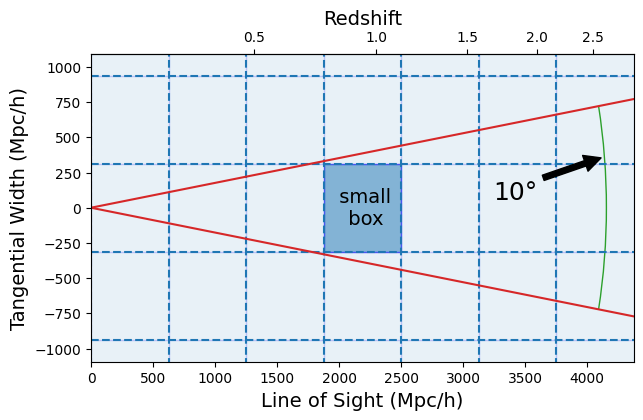
\includegraphics[width=0.8\textwidth]{figures/light_cone_configuration.png}
    \caption{Spatial and redshift setup for the \textbf{BIGBOX} and \textbf{TILED} simulations. Dashed blue grids partition the overall simulation volume into smaller, manageable tiling regions where each tile is a replication of the TILED simulation. The lower horizontal axis represents the line-of-sight distance measured in $\mathrm{Mpc}/h$, with the corresponding redshift values displayed on the top axis.} \label{fig:simulationsetting}
\end{figure}

Both simulations commence at an initial redshift of $z = 9$, utilizing an initial linear matter power spectrum at $z = 0$ generated via the \texttt{CLASS} code \citep{2011JCAP...07..034B}. We evolved the simulations over $60$ time steps, reaching the present day ($z = 0$). The resulting particle distribution are returned in $80$ shells taken from scale factor $a = 0.2$ to $a = 1.0$ with a uniform spacing of $\Delta a = 0.01$. At each scale factor $a_i$ on the fly, particles inside the shells are projected onto a HEALPix grid \citep{Górski_2005} with $N_{\text{side}} = 8192$, providing an angular resolution of approximately $0.43$ arcmin, to create mass maps. 

Note that the observer point is set at the corner point shared by $8$ replications for both TILED and BIGBOX simulations. This choice leads to Kaleidoscope pattern (see Figure~\ref{fig:boxreplication_patch}), existence of heavily tiled regions along the line of sight and near the equator, especially the direction which the box side and the line of sight are parallel. We will exclude the most heavily tiled regions in the analysis and discuss the Box Replication Effect in Section~\ref{sec:boxreplication}. 

\begin{figure}[ht]
    \centering
    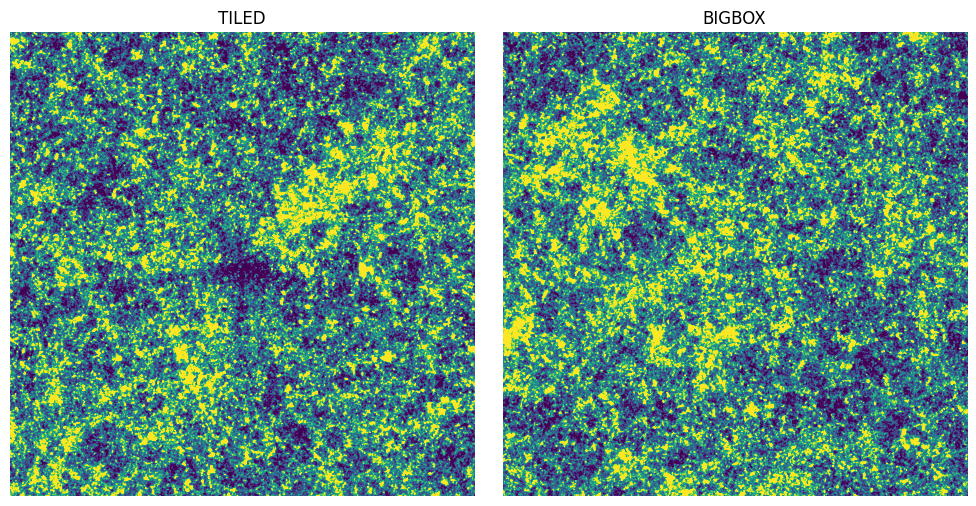
\includegraphics[width=\textwidth]{figures/samplepatch.png}
    \caption{Illustration of $5 \times 5$ patch around $(\theta, \phi)= (\pi/2, 0)$ extracted from TILED and BIGBOX simulations. A Kaleidoscope pattern is observed in the TILED simulation, while the BIGBOX simulation exhibits a more uniform distribution.} \label{fig:boxreplication_patch}
\end{figure}

\section{Generating Convergence Maps}
Since we already have the projected mass map at each scale factor, we can calculate the convergence map at each redshift following the discussion in Section~\ref{sec:convergence} and~\ref{sec:weak-lensing-generation}. Since the difference between TILED and BIGBOX simulations due to the super-sample effect shows up at the redshift $z \approx 1$, it is worthful to check the constribution from each redshift to the convergence map.

Figure~\ref{fig:lensing_efficiency} presents the normalized lensing efficiency as a function of comoving distance (measured in Mpc/$h$) for multiple source redshifts ($z$). The lensing efficiency curves exhibit peaks at intermediate comoving distances, indicating the regions where the distribution of matter along the line of sight most significantly enhances the gravitational lensing signal. 

\begin{figure}
    \centering
    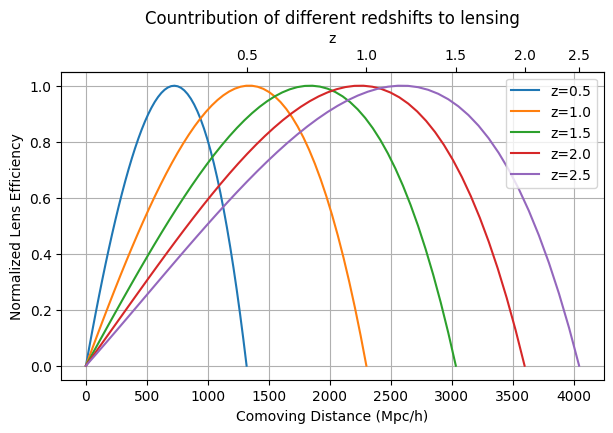
\includegraphics[width=0.8\textwidth]{figures/lensefficiency.png}
    \caption{Normalized lensing efficiency as a function of comoving distance for multiple source redshifts. The lensing efficiency peaks at intermediate comoving distances, indicating regions where the distribution of matter enhances the gravitational lensing signal.} \label{fig:lensing_efficiency}
\end{figure}

We considered source redshifts $z_s = [0.5, 1.0, 1.5, 2.0, 2.5]$ covering the range of distances relevant for current and future galaxy surveys. At redshift $z < 1$, both simulation suffer from the super-sample effect, while at redshift $z > 1$, the effect is more pronounced in the BIGBOX simulation. Figure~\ref{fig:convergence_maps} illustrates the convergence maps generated from the BIGBOX and TILED simulations for source redshift $z_s = 1.5$. 

\begin{figure}
    \centering
    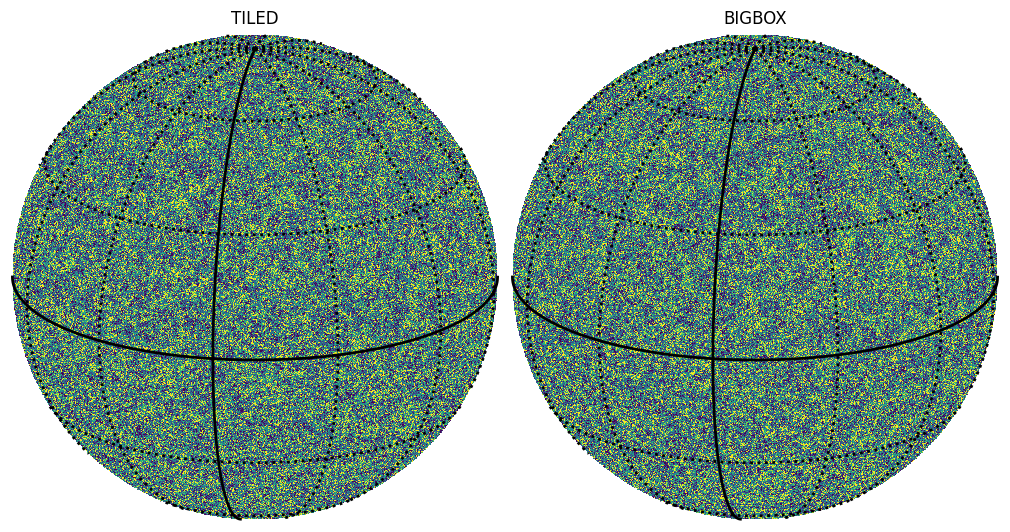
\includegraphics[width=\textwidth]{figures/samplemap.png}
    \caption{Convergence maps generated from the BIGBOX and TILED simulations for source redshift $z_s = 1.5$. The yellow regions represent positive convergence, while the blue regions indicate negative convergence. The convergence maps exhibit similar large-scale structures.} \label{fig:convergence_maps}
\end{figure}


\section{Incorporating Noise}
In real observations, measurements of the lensing signal are contaminated by noise arising from the intrinsic shapes of galaxies and errors in shape measurements. This noise, referred to as shape noise, constitutes a significant source of uncertainty, particularly on small angular scales.

We considered four different surveys with varying galaxy number densities, as detailed in Table~\ref{tab:survey_comparison}.
The variance of the shape noise per pixel was calculated as:
\begin{equation}
    \sigma_{\kappa, \text{noise}}^2 = \frac{\sigma_{\epsilon}^2}{2 n_{\mathrm{gal}} A_{\mathrm{pix}}},
\end{equation}
where $\sigma_{\epsilon}$ is the intrinsic ellipticity dispersion of galaxies, set to $\sigma_{\epsilon} = 0.26$ \citep{2019A&A...627A..59E}, $n_{\mathrm{gal}}$ is the galaxy number density per square arcminute, and $A_{\mathrm{pix}}$ is the solid angle of a pixel, set to $0.43$ arcminutes$^2$.
We generated a Gaussian random field $n(\hat{\mathbf{n}})$ with the calculated variance and added it to the convergence maps:
\begin{equation}
    \kappa_{\mathrm{obs}}(\hat{\mathbf{n}}) = \kappa(\hat{\mathbf{n}}) + n(\hat{\mathbf{n}}).
\end{equation}

\section{Patch Extraction for Analysis}
In order to simlplify the analysis onto a flat patch, we extracted patches from the full-sky convergence maps. Each patch covers an area of $10^\circ \times 10^\circ$ and is uniformly distributed across the sky using a Fibonacci grid \citep{2006QJRMS.132.1769S, 2023MNRAS.524.5591F}. The center of each patch is positioned at the vertices of the Fibonacci grid defined by golden ratio spirals:
\begin{equation}
    \sin \theta_i = \frac{2i}{2N + 1}, \quad \phi_i = \frac{2 \pi i}{\varphi}, \quad -N \leq i \leq N, \quad -\frac{\pi}{2} \leq \theta_i \leq \frac{\pi}{2},
\end{equation}
where $N$ is the number of patches and $\varphi = (1 + \sqrt{5})/2$ is the golden ratio. The visualization of the Fibonacci grid is shown in Figure~\ref{fig:fibonacci}.
\begin{figure}[ht]
    \centering
    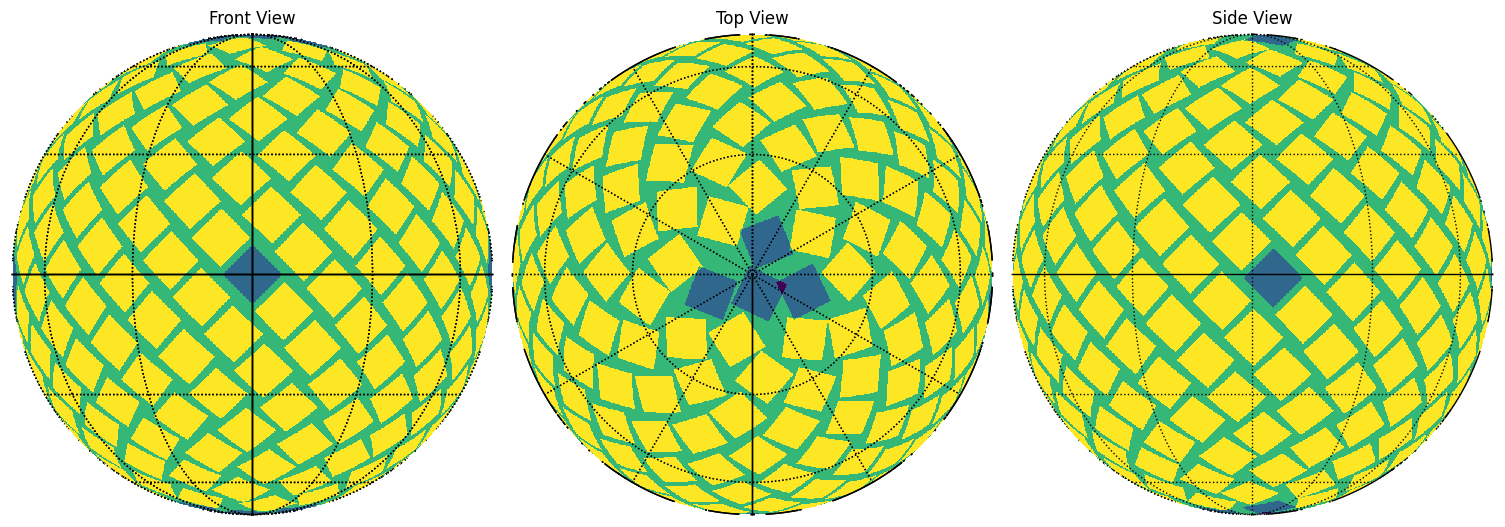
\includegraphics[width=\textwidth]{figures/fibonacci_grid.png}
    \caption{Visualization of the Fibonacci grid with $N_{\text{patches}} = 273$ patches, each covering approximately $10 \times 10$\,deg$^2$. 
    After the optimization and masking, the number of patches is reduced to $N_{\text{patches}} = 262$, effectively covering $64 \%$ of the sky.
    Each panel show the patches distribution on the Front, Top and Side view.}\label{fig:fibonacci}
\end{figure}

Figure~\ref{fig:fibonacci_extraction} showcases an extracted patch from the full-sky convergence map, and additional handling of the patches to get the desireed shape.

\begin{figure}
    \centering
    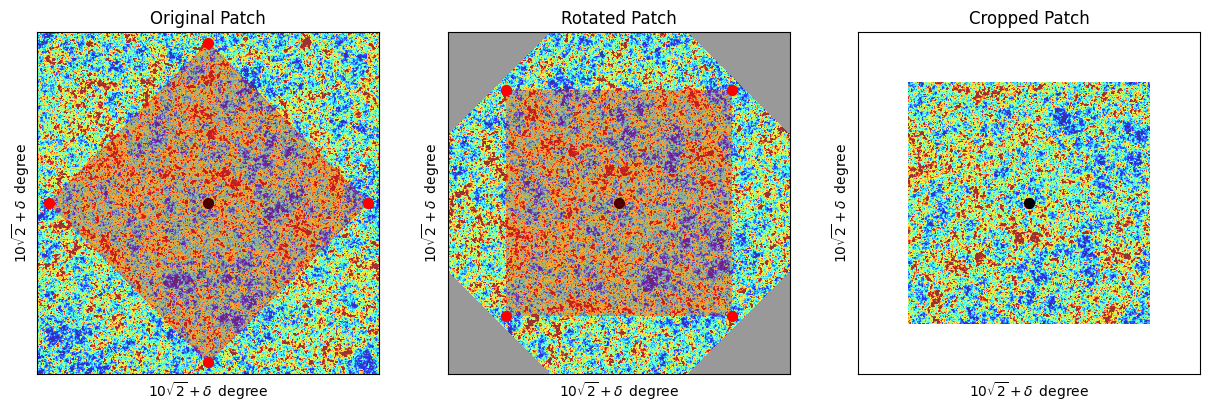
\includegraphics[width=\textwidth]{figures/fibonacci_extraction.png}
    \caption{Extraction of a patch from the full-sky convergence map using a Fibonacci grid. The patch covers an area of $10^\circ \times 10^\circ$ and is centered at the vertices of the Fibonacci grid. From the left to the right, the panels show the original extracted patch, patch rotated $45^\circ$ around the center and the final patch after the second rotation. The red shaded region represents the final patch we used for analysis.
    } \label{fig:fibonacci_extraction}
\end{figure}

Following \citet{2023MNRAS.524.5591F}, we can obtain the maximum number of patches by align the diagonal of square patches with the longitude lines. Nonetheless, we have to extract patches which their sides are aligned with the latitude lines due to the programming reason. Therefore, we first obtain a patch with wider side length and then rotate and crop the patch to get the desired shape.

For a Fibonacci grid center characterized by coordinates \( (\theta_i, \phi_i) \), we first employed the \texttt{gnomview} function from the \texttt{healpy} library \citep{Zonca2019} to project each spherical patch onto a flat plane via a gnomonic projection. Then for each patch, we rotated them by $45^\circ$ around the center of the patch to align the diagonal of the patch with the longitude lines. Finally, we cropped the patch according to the corresponding vertices:
\begin{align}
    \left( \theta_i - \Delta \theta,\, \phi_i - \Delta \phi \right), \quad &\left( \theta_i - \Delta \theta,\, \phi_i + \Delta \phi \right), \nonumber \\
    \left( \theta_i + \Delta \theta,\, \phi_i - \Delta \phi \right), \quad &\left( \theta_i + \Delta \theta,\, \phi_i + \Delta \phi \right),
\end{align}
with
\begin{align}
    \Delta \theta = 5\sqrt{2}\, \mathrm{\deg}, \quad \Delta \phi = 5\sqrt{2}\sin \theta_i \, \mathrm{\deg}.
\end{align}

The number of patches, denoted \( N_{\text{patches}} \), was optimized to ensure that individual patches do not overlap, except in regions near the poles where overlapping patches were subsequently discarded. The optimization process commenced with an initial count of \( N_{\text{patches}} = 400 \) and involved iteratively reducing this number until a configuration was achieved wherein the patches remained non-overlapping, except for centers located within \( 10\sqrt{2}^\circ \, \mathrm{\deg}\) of the poles, that is $|\theta_i| \geq 10\sqrt{2}^\circ$ and $|\phi_i| \leq \pi - 10\sqrt{2}^\circ$. Additionally, patches include points heavily tiled along with line of sight and near the equator are excluded to avoid severe Box Replication Effect (see Sec.~\ref{sec:boxreplication} for further check).

After optimization and masking, the number of patches was set to $N_{\text{patches}} = 273$, effectively reducing to $N_{\text{patches}} = 262$, effectively cover $64 \%$ of the sky. 
Each patch is represented by a $2048 \times 2048$ grid of pixels, resulting in a pixel size of:
\begin{equation}
    \Delta \theta = \frac{10^\circ}{2048} \approx 0.00488^\circ \approx 0.293' \quad \text{per pixel}.
\end{equation}
For each realization, the covariance is computed using 262 patches extracted from the full-sky map of each simulation.
Therefore, we obtain a total of 2882 patches from the BIGBOX simulation and 5240 patches from the TILED simulation. 

\section{Gaussian Smoothing}
Shape noise predominantly affects small angular scales. To mitigate this noise and enhance the detection of the underlying lensing signal, we applied Gaussian smoothing to the noisy convergence maps. The Gaussian filter used is defined by:
\begin{equation}
    W(\theta) = \frac{1}{\pi \theta_{\mathrm{G}}^2} \exp\left( -\frac{\theta^2}{\theta_{\mathrm{G}}^2} \right),
\end{equation}
where $\theta$ is the angular distance from the center of the filter, and $\theta_{\mathrm{G}}$ is the smoothing scale. For our analysis, we selected $\theta_{\mathrm{G}} = 2'$, $5'$, $8'$, and $10'$.

By convolving the noisy convergence map with the Gaussian filter, we obtained the smoothed convergence map:
\begin{equation}
    \kappa_{\mathrm{smoothed}}(\hat{\mathbf{n}}) = \int d\Omega' \, W(|\hat{\mathbf{n}} - \hat{\mathbf{n}}'|) \kappa_{\mathrm{obs}}(\hat{\mathbf{n}}').
\end{equation}

Figure~\ref{fig:smoothing} demonstrates the application of Gaussian smoothing to a noisy convergence map. The figure presents four panels, each corresponding to a different smoothing scale: $\theta_{\mathrm{G}} = 2'$, $5'$, $8'$, and $10'$. As the smoothing scale increases, the convolution with the Gaussian filter effectively reduces small-scale noise, as evidenced by the diminishing small-scale fluctuations in the map. 
\begin{figure}[ht]
    \centering
    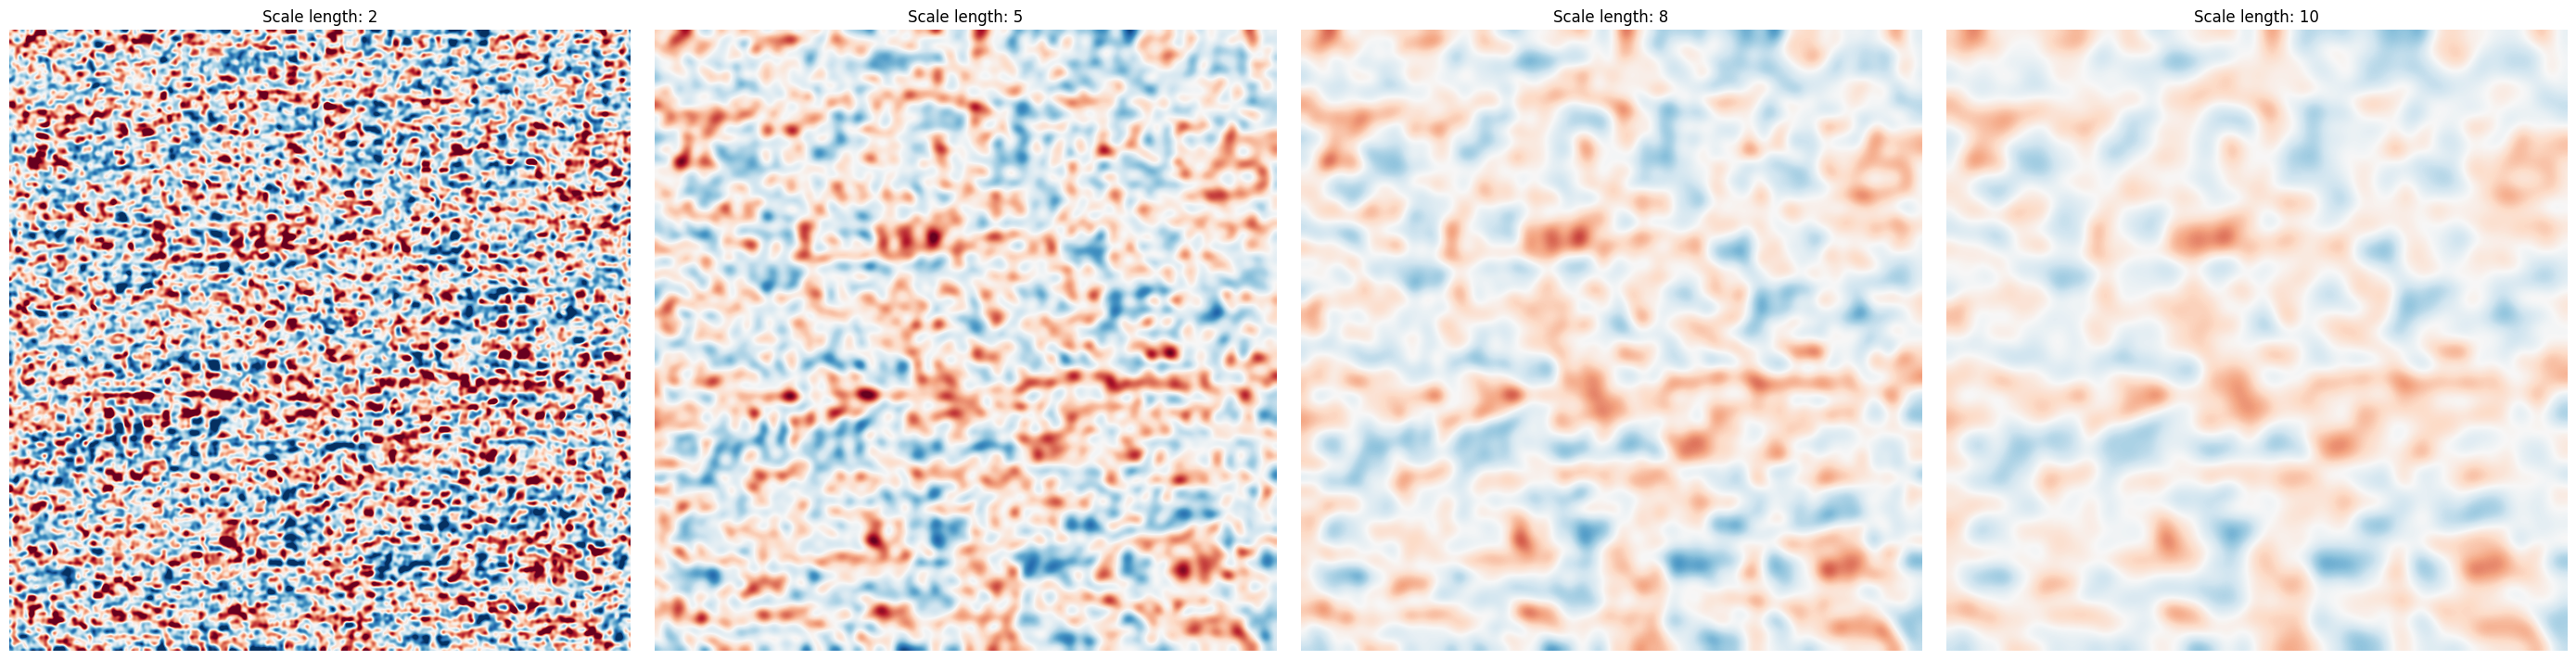
\includegraphics[width=\textwidth]{figures/smoothed_comparison.png}
    \caption{Effect of Gaussian smoothing on a noisy convergence map. Each panel shows the result of applying a Gaussian filter with a different smoothing scale $\theta_{\mathrm{G}} = 2'$, $5'$, $8'$, and $10'$. As the smoothing scale increases, small-scale noise is progressively suppressed, and large-scale structures become more prominent. This demonstrates how Gaussian smoothing effectively reduces shape noise while enhancing the detection of the underlying lensing signal.}
\label{fig:smoothing}
\end{figure}

For the non-Gaussian statistics, we adapt Gaussian smoothing. The statistics are then calculated from the smoothed convergence maps. The application of smoothing kernel to the convergence maps wash out the small-scale structures and therefore change the range of $\kappa$ values. To avoid the smoothing issues and the complex binning to consider, we normalize $\kappa$ values by the standard deviation of each patch's convergence map, $\sigma_{\kappa}$. Figure~\ref{fig:avg_sigma0} shows the average standard deviation of the noiseless convergence maps for the BIGBOX and TILED simulations. Obiviously, the standard deviation of convergence maps goes higher as the redshift or the smoothing scale decreases, while subtle difference between the BIGBOX and TILED simulations can be observed.

\begin{figure}[ht]
    \centering
    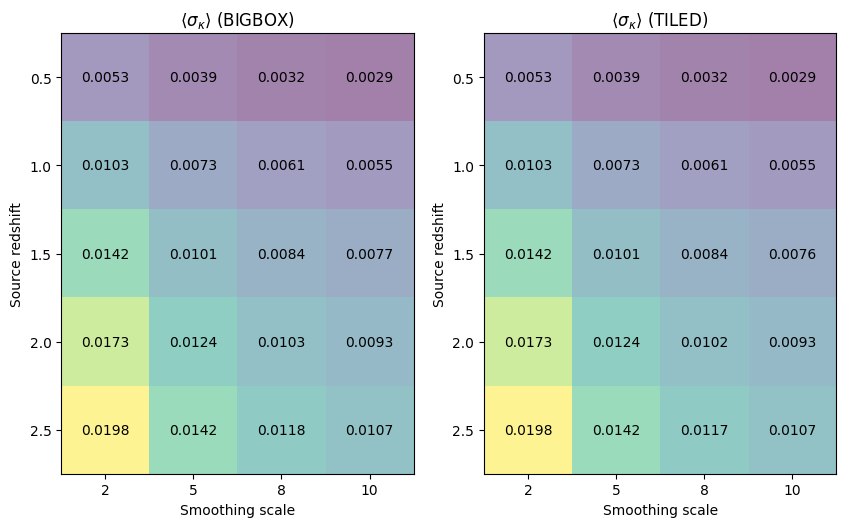
\includegraphics[width=\textwidth]{figures/avg_sigma0.png}
    \caption{Average standard deviation of the noiseless convergence maps for the BIGBOX and TILED simulations. The standard deviation increases with redshift and smoothing scale, with a subtle difference between the BIGBOX and TILED simulations.} \label{fig:avg_sigma0}
\end{figure}

\section{Measurements}
In order to characterize the influence of super-sample covariance on higher-order statistics, this study concentrates on the bispectrum, probability distribution function (PDF), peak counts, minima counts, and Minkowski functionals. 

Table~\ref{tab:statistics} delineates the range of values and the computational subroutines employed for each statistical measure. Each statistic is computed both for full-sky analyses and sky patches, utilizing the appropriate methodologies as specified.
\begin{table*}[htbp]
    \centering
    \begin{tabular}{lcc}
    \toprule
    \textbf{Statistic} & \textbf{Range} & \textbf{Subroutine (Sky Patch)} \\
    \midrule
    Angular Power Spectrum & $300 \leq \ell \leq 3000$ & \texttt{lenstools.powerSpectrum} \\
    Bispectrum & $300 \leq \ell \leq 3000$ & \texttt{lenstools.bispectrum} \\
    Peak Counts & $-4 \leq \kappa/\sigma_\kappa \leq 4$ & \texttt{lenstools.peakCount} \\
    Minima Counts & $-4 \leq \kappa/\sigma_\kappa \leq 4$ & \texttt{lenstools.peakCount} \\
    Probability Distribution Function (PDF) & $-4 \leq \kappa/\sigma_\kappa \leq 4$ & \texttt{lenstools.pdf} \\
    Minkowski Functionals & $-4 \leq \kappa/\sigma_\kappa \leq 4$ & own implementation \\
    \bottomrule
    \end{tabular}
    \caption{Summary of the statistical measures employed in this investigation, including their respective value ranges and computational subroutines utilized for both full-sky and sky-patch analyses.}\label{tab:statistics}
\end{table*}

\subsection{Angular Power Spectrum}
The angular power spectrum ($C_{\ell}^{\kappa\kappa}$) is calculated directly from the simulated convergence maps using \texttt{lenstools} \citep{2016A&C....17...73P} without performing any prior smoothing of the maps. We consider an angular multipole range from $\ell = 300$ to $\ell = 3000$ with $8$ logarithmically spaced bins. The number of bins is chosen to match the multipole selection in the HSC Y3 cosmic shear analysis \citep{2023PhRvD.108l3519D}. As the goal of this work is to investigate higher-order statistics, we choose the lower limit of $\ell = 300$ to avoid the large-scale regimes. The upper limit of $\ell = 3000$ is selected to ensure that the analysis reach the small-scale regime where the super-sample effect is more pronounced.

For a reference, we compute the theoretical prediction using \texttt{Halofit} \citep{2012ApJ...761..152T} and compare it with the measured angular power spectrum. 
The theoretical prediction is calculated using the same cosmological parameters as the simulations. 

\subsection{Bispectrum}
The bispectrum ($B_{\ell_1\ell_2\ell_3}^{\kappa\kappa\kappa}$) is computed from the unsmoothed convergence maps using \texttt{lenstools}. We consider three distinct configurations: equilateral ($\ell_1 = \ell_2 = \ell_3$), squeezed ($\ell_1 = \ell_2 = 10\ell_3$), and isosceles ($\ell_1 = \ell_2 = 2\ell_3$). 
Those configurations are chosen to capture the different shapes of the bispectrum and provide complementary information about the underlying matter distribution.
The bispectrum calculations are confined within the multipole range $\ell \in [300, 3000]$ with $8$ logarithmically spaced bins, same as the angular power spectrum. Though the bispectrum is more senstive to the noise and the small-scale structures, we choose the same multipole range to compare the results with the angular power spectrum.

For the bispectrum, we also compute the theoretical prediction using the \texttt{BiHalofit} code~\citep{2020ApJ...895..113T} and compare it with the measured bispectrum. The theoretical prediction is calculated using the same cosmological parameters as the simulations.

\subsection{PDF}
The PDF of the convergence field is computed from the smoothed convergence maps using \texttt{lenstools}. The PDF is calculated within the normalized range $-4 \leq \kappa/\sigma_{\kappa} \leq 4$, linearly divided into 8 bins. $\sigma_{\kappa}$ denotes the standard deviation of each patch's convergence map.

The thoretical prediction for the PDF is calculated using the \texttt{hmpdf} code~\cite{2020PhRvD.102l3545T} and compared with the measured PDF. The theoretical prediction is calculated based on the same linear matter power spectrum as the simulations.

\subsection{Peak/Mimina Counts}
The peak and minima counts are computed from the smoothed convergence maps using \texttt{lenstools}. The peak and minima counts are calculated within the normalized range $-4 \leq \kappa/\sigma_{\kappa} \leq 4$, linearly divided into 8 bins. Thought the highest/lowest peaks contain only few data points, we choose to include them in the analysis to match the range of the PDF.

\subsection{Minkowski Functionals}
The Minkowski functionals are computed from the smoothed convergence maps using our own implementation naively follow the definition in Section~\ref{sec:minkowski_functionals}. They are calculated within the normalized range $-4 \leq \kappa/\sigma_{\kappa} \leq 4$, linearly divided into 8 bins. We show $\sigma_1 = \sqrt{\kappa_{x}^2 + \kappa_{y}^2}$ which used to calculate the Minkowski functionals in Figure~\ref{fig:avg_sigma1}. The values decrease as the smoothing scale increases, while the difference between the BIGBOX and TILED simulations or the redshifts is subtle.

\begin{figure}[ht]
    \centering
    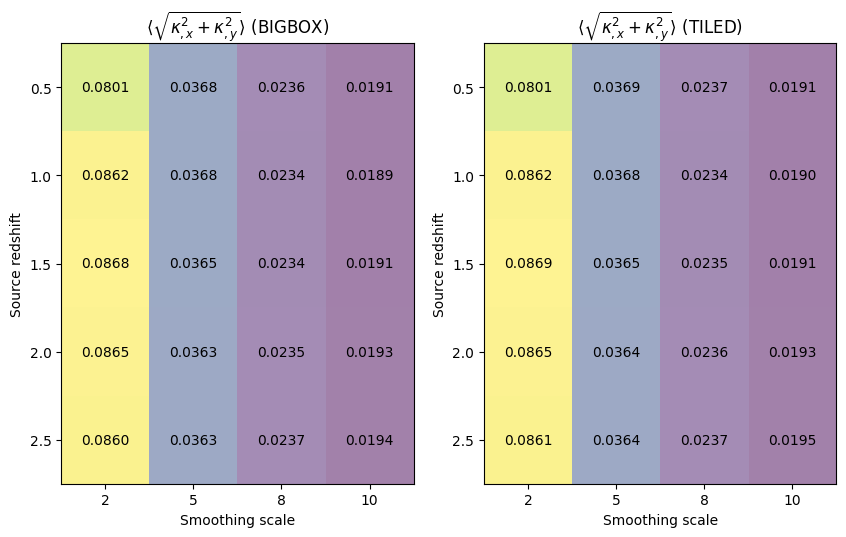
\includegraphics[width=\textwidth]{figures/avg_sigma1.png}
    \caption{Average $\sigma_1 = \sqrt{\kappa_{x}^2 + \kappa_{y}^2}$ of the noiseless convergence maps for the BIGBOX and TILED simulations. They are calculated for the smoothing scales $\theta_{\mathrm{G}} = 2'$, $5'$, $8'$, and $10'$. The values decrease as the smoothing scale increases, while the difference between the BIGBOX and TILED simulations or the redshifts is subtle.
    } \label{fig:avg_sigma1}
\end{figure}

\subsection{Covariance Matrix Estimation}
Following the measurement phase, this study examines the influence of super-sample covariance on the covariance matrices associated with the aforementioned statistical measures. To achieve this, we employ an unbiased estimator for the covariance matrix as previously defined in Equation~\ref{eq:covariance}. 

Additionally, we also compute the correlation matrix for each statistical measure to investigate the interdependence between different scales and configurations. The correlation matrix is defined as:
\begin{equation}
    \rho_{ij} = \frac{\text{Cov}(\mathcal{O}_i, \mathcal{O}_j)}{\sqrt{\text{Cov}(\mathcal{O}_i, \mathcal{O}_i)\text{Cov}(\mathcal{O}_j, \mathcal{O}_j)}},
\end{equation}
where $\mathcal{O}_i$ and $\mathcal{O}_j$ represent the $i$-th and $j$-th statistical measures, respectively.

After the covariance and correlation matrices are computed for both the BIGBOX and TILED simulations, we compare the matrices to quantify the impact of super-sample covariance on the statistical measures. The comparison is conducted by calculating the ratio between the covariance and correlation matrices of the BIGBOX and TILED simulations. 

In the case of correlation matrices, we exclude the diagonal elements---since they are always unity---when calculating the ratio. For covariance matrices, the ratio is calculated over the entire matrix. 

Regarding $\ell$-binned statistics, we determine the ratio across all bins. For $\nu$-binned statistics, we exclude the first and last bins from the ratio calculation due to their limited data points and unreliability.